\documentclass{article}
\usepackage[utf8]{inputenc}
\usepackage{graphicx}
\title{Assignment 4 Project Management Agile Development}
\author{peter }
\date{August 2019}

\begin{document}

\maketitle

\section{Team Members}
BHAGAT SINGH (C0735947)\\
Robanpreet Kaur Randhawa  (C0737536)\\
Anshpreet Kaur Randhawa(C0737534)\\
Kiranbir Kaur(C0740055)\\
Jagroop Singh (C0739304)\\
Paras Kumar (C0737465)\\
\section *{Screenshot for page 1}
\includegraphics[width=20cm]{1.PNG}
\section *{Screenshot for page 2}
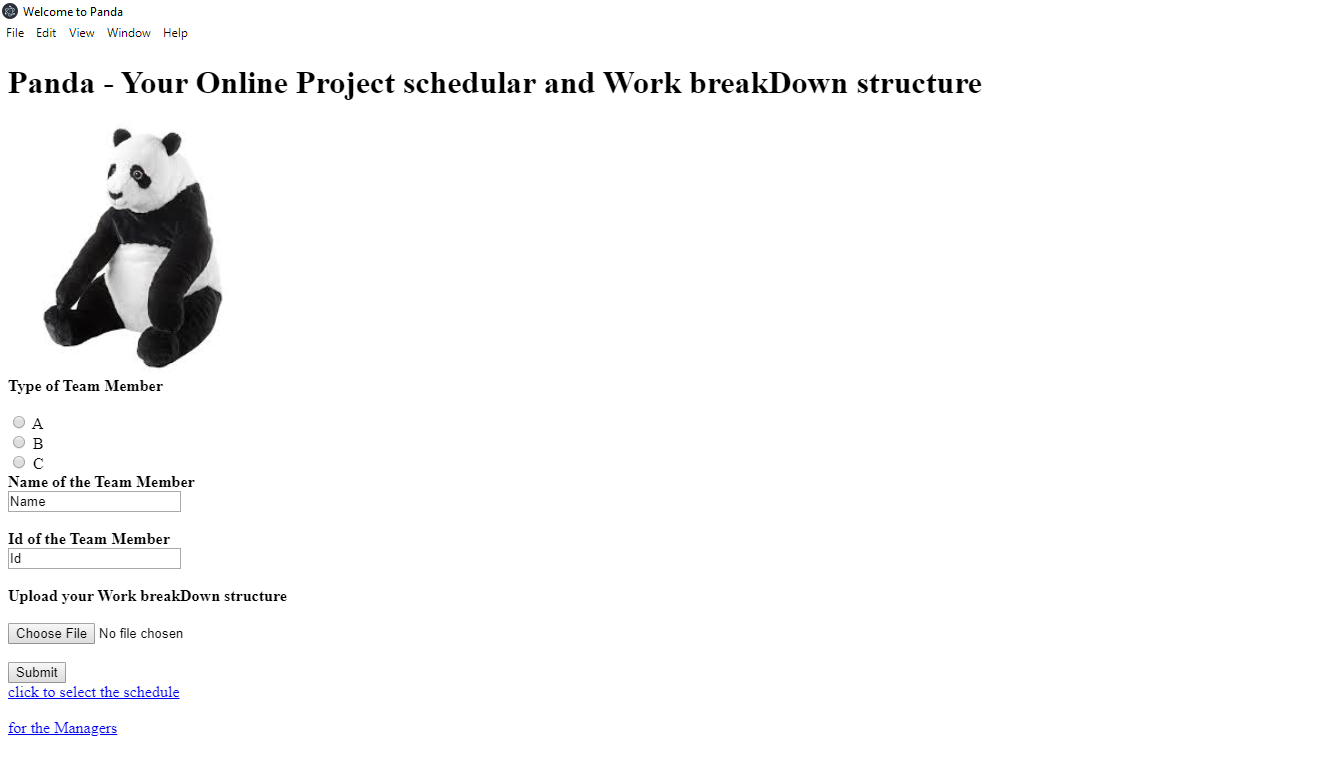
\includegraphics[width=20cm]{2.PNG}
\section *{Screenshot for page 3}
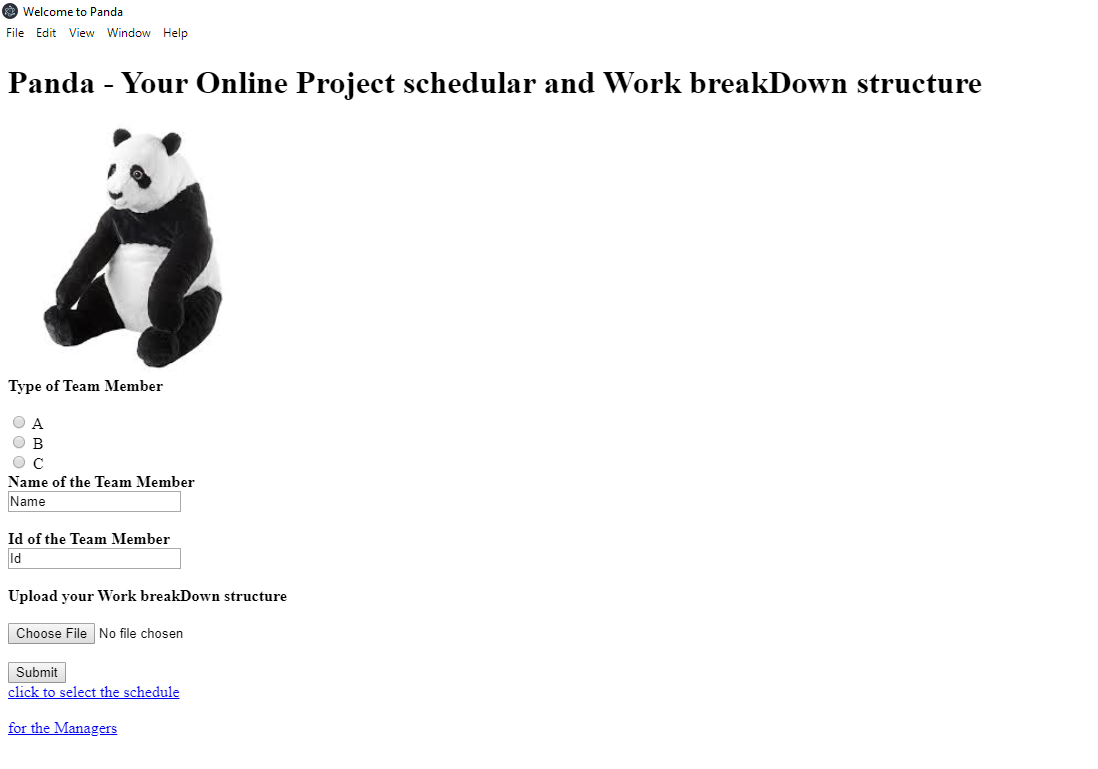
\includegraphics[width=20cm]{3.PNG}
\section * {Our Web Application Code:}
\section *{Code for page 1}
\begin{verbatim}

<!DOCTYPE html>
<html>
  <head>
    <meta charset="UTF-8">
    <title>Welcome to Panda</title>
    <script>
      function a() = {
 }
    </script>
  </head>
  <body onload='a()'>
    <h1>Panda - Your Online Project schedular and Work breakDown structure</h1>
    
    <img src='\\storage\storage$\737536\Documents\panda.jpg' width = '250' />
    
<form>
    <label for="uname"><b>Type of Team Member   </b></label><br><br>
    <input type="radio" name="type" value="A"> A <br>
    <input type="radio" name="type" value="B"> B <br>
    <input type="radio" name="type" value="C"> C </br>
    <label for="uname"><b>Name of the Team Member  </b></label></br>
    <input type="text" width='200' value="Name"></br> </br>
    <label for="uname"><b>Id of the Team Member    </b></label></br>
    <input type="text" width='200' value="Id"></br> </br>

  <form action="/action_page.php">
    <label for="uname"><b>Upload your Work breakDown structure  </b></label></br></br>
    <input type="file" name="pic" accept="image/*"></br></br>
    <input type="submit" value= "Submit" >
  </form>

  
</form>

    <!-- You can also require other files to run in this process -->
    <script src="./renderer.js"></script>


    <a href="/electron-quick-start/page2.html">click to select the schedule</a href></br> </br>
      <a href="/electron-quick-start/page3.html">for the Managers</a href>
  </body>
  
</html>



\end{verbatim}
\section *{Code for page 2}
\begin{verbatim}

<!DOCTYPE html>
<html>
  <head>
    <meta charset="UTF-8">
    <title>Welcome to Panda</title>
    <script>
      function a() = {
    }
    </script>
  </head>
  <body onload='a()'>
    <h1>Panda - Your Online Project schedular and Work breakDown structure</h1>
    
    <img src='\\storage\storage$\737536\Documents\panda.jpg' width = '250' />
    
<form>
    <label for="uname"><b>Type of Team Member   </b></label><br><br>
    <input type="radio" name="type" value="A"> A <br>
    <input type="radio" name="type" value="B"> B <br>
    <input type="radio" name="type" value="C"> C </br>
    <label for="uname"><b>Name of the Team Member  </b></label></br>
    <input type="text" width='200' value="Name"></br> </br>
    <label for="uname"><b>Id of the Team Member    </b></label></br>
    <input type="text" width='200' value="Id"></br> </br>

    <label for="uname"><b>Enter your idea   </b></label></br>
    <textarea rows="4" cols="50">
       keep your idea to 100 words
    </textarea>
 
</br></br>
<label for="uname"><b>Select your schedule  </b></label>
  <select>
      <option value="volvo"> 8am to 2pm </option>
      <option value="saab"> 2pm to 8pm </option>
      <option value="opel"> 8pm to 1am </option>
      <option value="audi"> 1am to 8am </option>
    </select>
  </br></br>
  <input type="submit" value= "Submit" >
  
</form>

    <!-- You can also require other files to run in this process -->
    <script src="./renderer.js"></script>
    <a href="/electron-quick-start/index.html">click to upload your work breakDown structure</a href></br> </br>
      <a href="/electron-quick-start/page3.html">for the Managers</a href>
  </body>
  
</html>




\end{verbatim}
\section *{Code for page 3}
\begin{verbatim}

<!DOCTYPE html>
<html>
  <head>
    <meta charset="UTF-8">
    <title>Welcome to Panda</title>
    <script>
      function a() = {

    </script>
  </head>
  <body onload='a()'>
    <h1>Panda - Your Online Project schedular and Work breakDown structure</h1>
    
    <img src='\\storage\storage$\737536\Documents\panda.jpg' width = '250' />
    
<form>
    
    <label for="uname"><b>Name of the Manager  </b></label></br>
    <input type="text" width='200' value="Name"></br> </br>
    <label for="uname"><b>Id of the Manager    </b></label></br>
    <input type="text" width='200' value="Id"></br> </br>

  <form action="/action_page.php">
    <label for="uname"><b>Upload your Project   </b></label></br>
    <input type="file" name="pic" accept="image/*"></br></br>
    <input type="submit" value= "Submit" >
  </form>
</br></br>
  <label for="uname"><b>Suggestion to the project  </b></label></br>
    <textarea rows="4" cols="50">
       keep your suggestions to 100 words
    </textarea>
  </br></br>

    <input type="submit" value= "Approval" ></br> </br>
  
</form>

    <!-- You can also require other files to run in this process -->
    <script src="./renderer.js"></script>
   
      <a href="/electron-quick-start/index.html"> click if you are an employee </a href>
        
  </body>
  
</html>



\end{verbatim}

\end{document}